\begin{frame}
	\frametitle{Impostos Indirectos}
	\begin{itemize}
		\setlength{\itemsep}{0.2cm}
		\item \textbf{Espec\'ificos:} O Governo cobra aos produtores uma certa import\^ancia fixa por cada unidade oferecida e vendida:
		\begin{itemize}
			\item Imposto sobre Ve\'iculos (ISV)
			\item Imposto sobre os Combust\'iveis (ISP)
		\end{itemize}
		\item \textbf{ad valorem:} o Governo cobra um valor que corresponde a uma percentagem aplicada ao pre\c co do produto:
		\begin{itemize}
			\item Imposto sobre o Valor Acrescentado (IVA)
		\end{itemize}
	\end{itemize}

\end{frame}

\begin{frame}
	\frametitle{Impostos Indirectos}
	\begin{itemize}
		\item O la\c camento de um imposto faz com que o pre\c co que o consumidor paga seja diferente do pre\c co que o produtor recebe numa transac\c c\~ao, ou seja: \[P_d=P_s+imposto\]
		\item Aos olhos do consumidor, a oferta apresentar-se-\`a distorcida, porque pagar\'a cada unidade mais cara...
	\end{itemize}
	\begin{center}
		Normalmente, \'e o produtor que tem a responsabilidade de cobrar o imposto e entregar o valor ao Estado (incid\^encia legal do imposto), mas veremos que o imposto tem incid\^encia econ\'omica em ambos os lados do mercado.
	\end{center}
\end{frame}

\begin{frame}
	\frametitle{Impostos Indirectos}
	O equil\'ibrio de mercado ap\'os introdu\c c\~ao do imposto \'e sempre caraterizado por:
	\begin{align*}	
		\left\{
		\begin{array}{c}
			Q_D=f_d(P_d)\\
			Q_S=f_s(P_S)\\
			Q_D=Q_S
			\\P_d=P_s+I
		\end{array}\right.
	\end{align*}
	No caso de um imposto espec\'ifico, $I$ \'e uma constante; no caso de um imposto \emph{ad valorem} \`a taxa $t$, tem-se: \[I=t\times P_S\]
\end{frame}

\begin{frame}
	\frametitle{Exemplo: \(Q_D=100-P\), \(Q_S=3P\)}

	Equil\'ibrio de Mercado, sem interven\c c\~oes

	\begin{align*}
		\left\{
			\begin{array}{c}
				Q_D=100-P\\
				Q_S=3P\\
				Q_D=Q_S
			\end{array}
		\right.
		\Leftrightarrow
		\left\{
			\begin{array}{c}
				Q_D=Q_S=75\\
				P=25
			\end{array}
		\right.
	\end{align*}

	\begin{center}
		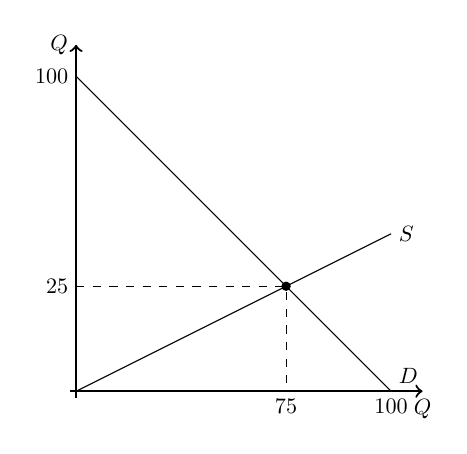
\begin{tikzpicture}[
			scale = 0.8,
			every node/.style = {scale = 0.8},
			declare function = {
				d(\x) = 5-\x;
				s(\x) = (1/2)*\x;
			}]

			\draw[->,thick] (-0.1,0) -- (5.5,0)node[below]{$Q$};
			\draw[->,thick] (0,-0.1) -- (0,5.5)node[left]{$Q$};

			\draw[domain=0:5,variable=\x] plot (\x,{d(\x)})node[above right]{$D$}node[below]{100};
			\draw[domain=0:5,variable=\x] plot (\x,{s(\x)})node[right]{$S$};

			\draw(0,{d(0)}) node[left]{100};

			\draw[dashed] (0,{5/3})node[left]{25} -- ({10/3},{5/3})node[circle,fill,inner sep=1.5]{} -- ({10/3},0)node[below]{75};

		\end{tikzpicture}
	\end{center}

\end{frame}

\begin{frame}
	\frametitle{Exemplo: \(Q_D=100-P\), \(Q_S=3P\)}
		Com lan\c camento de imposto espec\'ifico de 10um.
		\begin{align*}
			\left\{
				\begin{array}{c}
					Q_D=100-P_D\\
					Q_S=3P_S\\
					Q_D=Q_S\\
					P_D=P_S+10
				\end{array}
			\right.
			\Leftrightarrow
			\left\{
				\begin{array}{c}
					Q_D=Q_S=67.5\\
					P_D=32.5\\
					P_S=22.5
				\end{array}
			\right.
		\end{align*}

	\begin{center}
		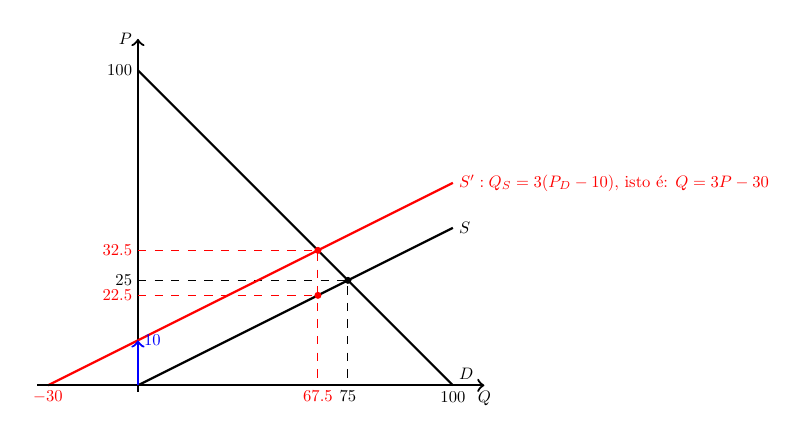
\begin{tikzpicture}[
			scale = 0.8,
			every node/.style = {scale = 0.6},
			declare function = {
				d(\x) = 5-\x;
				s(\x) = (1/2)*\x;
			}]

			\draw[->,thick] (-0.1,0) -- (5.5,0)node[below]{$Q$};
			\draw[->,thick] (0,-0.1) -- (0,5.5)node[left]{$P$};

			\draw[domain=0:5,variable=\x,thick] plot (\x,{d(\x)})node[above right]{$D$}node[below]{100};
			\draw[domain=0:5,variable=\x,thick] plot (\x,{s(\x)})node[right]{$S$};

			\draw(0,{d(0)}) node[left]{100};

			\draw[dashed] (0,{5/3})node[left]{25} -- ({10/3},{5/3})node[circle,fill,inner sep=1.5]{} -- ({10/3},0)node[below]{75};

			\onslide<2->{
				\draw[dashed,red] (0,{d(10/3.5)})node[left]{32.5} -- ({10/3.5},{d(10/3.5)}) node[circle,fill=red,inner sep=1.5]{} -- ({10/3.5},0)node[below]{67.5};
				\draw[dashed,red] (0,{s(10/3.5)})node[left]{22.5} -- ({10/3.5},{s(10/3.5)}) node[circle,fill=red,inner sep=1.5]{};
			}

			\onslide<3->{
				\draw[domain=0:5,variable=\x,thick,red] plot (\x,{s(\x)+(d(10/3.5)-s(10/3.5))}) node[right]{$S':Q_S=3(P_D-10)$, isto \'e: $Q=3P-30$};
			}

			\onslide<4->{
				\draw[domain={-2*(d(10/3.5)-s(10/3.5))}:0,variable=\x,thick,red] plot (\x,{s(\x)+(d(10/3.5)-s(10/3.5))});
				\draw[thick] (-1.6,0) -- (-0.1,0);
				\draw[red]({-2*(d(10/3.5)-s(10/3.5))},0)node[below]{$-30$};
			}

			\onslide<5->{
				\draw[thick,->,blue] (0,0) -- (0,{(d(10/3.5)-s(10/3.5))})node[right]{10};
			}

		\end{tikzpicture}
	\end{center}

\end{frame}

\begin{frame}
	\frametitle{Observa\c c\~oes:}
	\begin{itemize}
		\item A oferta n\~ao sofreu uma contrac\c c\~ao $S\parallel S'$!
		\item<2-> A oferta $S'$ \'e aquela que \'e vista pelo consumidor, j\'a que estamos a admitir que o imposto \'e recolhido e entregue ao Estado pelo produtor (incid\^encia legal do imposto)
		\item<3-> A oferta $S'$, aos olhos do consumidor, encontra-se distorcida face \`a oferta de mercado, que continua a ser $S$
		\item <4-> Os impostos indiretos s\~ao DISTORCION\'ARIOS
	\end{itemize}
\end{frame}

\begin{frame}
	\frametitle{Impostos Indirectos (imposto espec\'ifico)}
	\begin{center}
		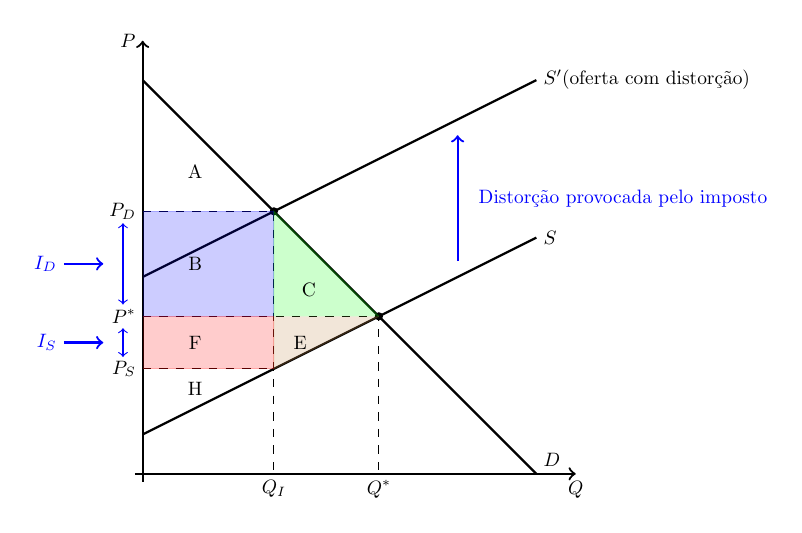
\begin{tikzpicture}[
			scale = 1,
			every node/.style = {scale = 0.7},
			declare function = {
				sa(\x) = 1/2 + 1/2 * \x;
				sb(\x) = 5/2 + 1/2 * \x;
				d(\x) = 5 - \x;
			}]

			\def\eqa{3}
			\def\eqb{5/3}

			\draw[->,thick] (-0.1,0) -- (5.5,0)node[below]{$Q$};
			\draw[->,thick] (0,-0.1) -- (0,5.5)node[left]{$P$};

			\draw[thick,domain=0:5,variable=\x] plot (\x,{d(\x)})node[above right]{$D$};
			\draw[thick,domain=0:5,variable=\x] plot (\x,{sa(\x)})node[right]{$S$};

			\onslide<2->{
				\draw[->,thick,blue] ({\eqa+1},{sa(\eqa+1)+0.2}) -- ({\eqa+1},{sb(\eqa+1)-0.2}) node[midway,xshift=3cm]{Distor\c c\~ao provocada pelo imposto};
				\draw[thick,domain=0:5,variable=\x] plot (\x,{sb(\x)})node[right]{$S'$(oferta com distor\c c\~ao)};
			}

			\onslide<3->{
				\draw[dashed] (0,{sa(\eqa)})node[left]{$P^*$} -- (\eqa,{sa(\eqa)})node[circle,fill,inner sep=1.5]{} -- (\eqa,0)node[below]{$Q^*$};
			}

			\onslide<4->{
				\draw[dashed] (0,{sb(\eqb)})node[left]{$P_D$} -- (\eqb,{sb(\eqb)})node[circle,fill,inner sep=1.5]{} -- (\eqb,0)node[below]{$Q_I$};
				\draw[dashed] (0,{sa(\eqb)})node[left]{$P_S$} -- (\eqb,{sa(\eqb)});
			}

			\onslide<5->{
				\draw[fill,opacity=0.2,blue] (0,{sa(\eqa)}) -- (\eqb,{sa(\eqa)}) -- (\eqb,{sb(\eqb)}) -- (0,{sb(\eqb)});
				\draw[fill,opacity=0.2,red] (0,{sa(\eqa)}) -- (\eqb,{sa(\eqa)}) -- (\eqb,{sa(\eqb)}) -- (0,{sa(\eqb)});
				\draw[fill,opacity=0.2,brown] (\eqb,{sa(\eqa)}) -- (\eqb,{sa(\eqb)}) -- (\eqa,{sa(\eqa)});
				\draw[fill,opacity=0.2,green] (\eqb,{sa(\eqa)}) -- (\eqb,{sb(\eqb)}) -- (\eqa,{sa(\eqa)});

				\draw({2/3},{(sb(\eqb)+d(2/3))/2})node[]{A};
				\draw({2/3},{(sa(2/3)+sa(\eqb))/2})node[]{H};
				\draw({2/3},{(sb(\eqb)+sa(\eqa))/2})node[]{B};
				\draw({2/3},{(sa(\eqb)+sa(\eqa))/2})node[]{F};
				\draw({\eqb+(\eqa-\eqb)/3},{(d((\eqa+\eqb)/2))+d(\eqa))/2})node[]{C};
				\draw({\eqb+(\eqa-\eqb)/4},{(sa(\eqb)+d(\eqa))/2})node[]{E};
			}

			\onslide<6->{
				\draw[thick,blue,->] (-1,{(sb(\eqb)+sa(\eqa))/2})node[left]{$I_D$} -- (-0.5,{(sb(\eqb)+sa(\eqa))/2});
				\draw[thick,blue,->] (-1,{(sa(\eqb)+sa(\eqa))/2})node[left]{$I_S$} -- (-0.5,{(sa(\eqb)+sa(\eqa))/2});
				\draw[<->,blue] (-0.25,{sa(\eqb)+0.15}) -- (-0.25,{sa(\eqa)-0.15});
				\draw[<->,blue] (-0.25,{sa(\eqa)+0.15}) -- (-0.25,{sb(\eqb)-0.15});
			}

		\end{tikzpicture}
	\end{center}
\end{frame}

\begin{frame}
	\frametitle{Em resumo...}
	\begin{center}
		{\renewcommand{\arraystretch}{1.5}
		\begin{tabular}{ccc}
			\rowcolor{iscal_color!50!white}& {\color{white}\textbf{Ap\'os imposto}} & {\color{white}\textbf{ Antes de imposto}} \\\hline
			\rowcolor{iscal_color!20!white}Excedente de Consumidor & $A$ & $A+B+C$ \\
			\rowcolor{iscal_color!10!white}Excedente de Produtor & $H$ & $F+E+H$ \\
			\rowcolor{iscal_color!20!white}Receita Fiscal (do Estado) & $B+F$ & -- \\
			\rowcolor{iscal_color!10!white}Perda Pura de Excedente & $C+E$ & -- \\
			\rowcolor{iscal_color!20!white}Quantidade Transaccionada & $Q_I$ & $Q^*$ \\
			\rowcolor{iscal_color!10!white}Pre\c co Transac\c c\~ao & $P_D$ ; $P_S$ & $P^*$
		\end{tabular}
		}
		\vskip 0.5cm
		Incid\^encia Econ\'omica do Imposto, por unidade transaccionada:\par $I_S$(produtor); $I_D$(consumidor)
	\end{center}
\end{frame}

\begin{frame}
	\frametitle{Em resumo no exemplo}
	\begin{columns}
		\begin{column}{0.5\textwidth}
			\begin{center}
				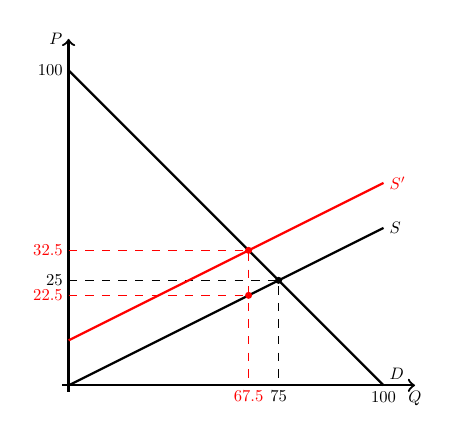
\begin{tikzpicture}[
					scale = 0.8,
					every node/.style = {scale = 0.6},
					declare function = {
						d(\x) = 5-\x;
						s(\x) = (1/2)*\x;
					}]

					\draw[->,thick] (-0.1,0) -- (5.5,0)node[below]{$Q$};
					\draw[->,thick] (0,-0.1) -- (0,5.5)node[left]{$P$};

					\draw[domain=0:5,variable=\x,thick] plot (\x,{d(\x)})node[above right]{$D$}node[below]{100};
					\draw[domain=0:5,variable=\x,thick] plot (\x,{s(\x)})node[right]{$S$};

					\draw(0,{d(0)}) node[left]{100};

					\draw[dashed] (0,{5/3})node[left]{25} -- ({10/3},{5/3})node[circle,fill,inner sep=1.5]{} -- ({10/3},0)node[below]{75};

					\draw[dashed,red] (0,{d(10/3.5)})node[left]{32.5} -- ({10/3.5},{d(10/3.5)}) node[circle,fill=red,inner sep=1.5]{} -- ({10/3.5},0)node[below]{67.5};
					\draw[dashed,red] (0,{s(10/3.5)})node[left]{22.5} -- ({10/3.5},{s(10/3.5)}) node[circle,fill=red,inner sep=1.5]{};

					\draw[domain=0:5,variable=\x,thick,red] plot (\x,{s(\x)+(d(10/3.5)-s(10/3.5))}) node[right]{$S'$};

				\end{tikzpicture}
			\end{center}
		\end{column}
		\begin{column}{0.4\textwidth}
			\(I_S=25-22.5=2.5um\)
			\(I_D=32.5-25=7.5um\)
			\(Total=10um=I\)
		\end{column}
	\end{columns}
\end{frame}

\begin{frame}
	\frametitle{Incid\^encia Econ\'omica}
	Quanto maior a elasticidade da procura (em m\'odulo) relativamente \`a da oferta, maior a incid\^encia do imposto sobre o lado da oferta.\par
	Pode demonstrar-se que:\[\frac{|\varepsilon_D|}{\varepsilon_S}=\frac{I_S}{I_D}\]
\end{frame}

\begin{frame}
	\frametitle{No exemplo}
		\begin{align*}
			Q_D=100-P&\rightarrow|\varepsilon_D|=\left|-1\times\frac{25}{75}\right| = 0.33\\
			Q_S=3P&\rightarrow\varepsilon_S=3\times\frac{25}{75}=1\\
			&\Downarrow\\
			\frac{|\varepsilon_D|}{\varepsilon_S}&=0.33\\
			\frac{I_S}{I_D}&=\frac{2.5}{7.5}=0.33
		\end{align*}
\end{frame}

\begin{frame}
	\frametitle{Elasticidade e Incid\^encia}
	\begin{align*}
		\frac{|\varepsilon_D|}{\varepsilon_S}&=\frac{I_S}{I_D}\\
		|\varepsilon_D|<\varepsilon_S\ &\Rightarrow\ I_D>I_S
	\end{align*}
\end{frame}

\begin{frame}
	\frametitle{Elasticidade e Incid\^encia}
	Quanto maior a elasticidade da procura (em m\'odulo) relativamente \`a da oferta, maior ser\'a a distor\c c\~ao da quantidade transacionada induzida pelo imposto (e, portanto, maior a perda de excedente econ\'omico).
\end{frame}

\begin{frame}
	\frametitle{Impostos Indirectos}
	A perda excedente econ\'omico (perda pura) \'e tanto menor quanto menor a elasticidade de um dos lados do mercado e, portanto, menor a dist\^ancia entre $Q^*$ e $Q_I$
	\begin{center}
		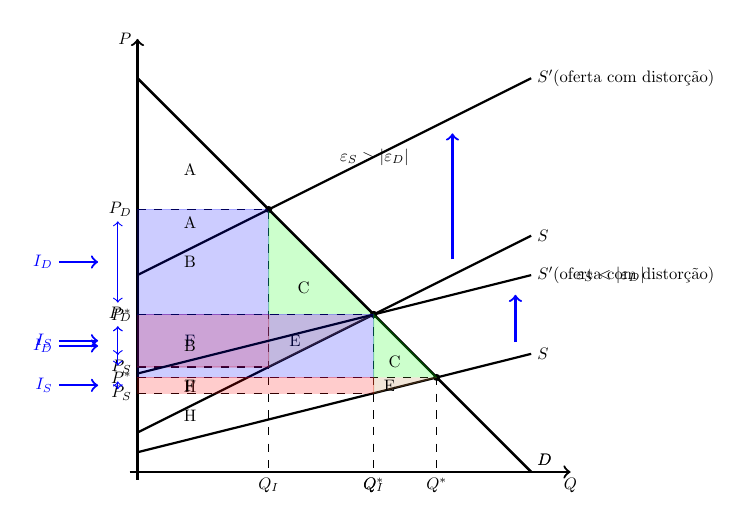
\begin{tikzpicture}[
			scale = 1,
			every node/.style = {scale = 0.6},
			declare function = {
				sa(\x) = 1/2 + 1/2 * \x;
				sb(\x) = 5/2 + 1/2 * \x;
				sc(\x) = 1/4 + 1/4 * \x;
				sd(\x) = 5/4 + 1/4 * \x;
				d(\x) = 5 - \x;
			}]

			\def\eqa{3}
			\def\eqb{5/3}
			\def\eqc{19/5}
			\def\eqd{3}

			\draw[->,thick] (-0.1,0) -- (5.5,0)node[below]{$Q$};
			\draw[->,thick] (0,-0.1) -- (0,5.5)node[left]{$P$};

			\onslide<1>{

				\draw[thick,domain=0:5,variable=\x] plot (\x,{d(\x)})node[above right]{$D$};
				\draw[thick,domain=0:5,variable=\x] plot (\x,{sa(\x)})node[right]{$S$};

				\draw[->,thick,blue] ({\eqa+1},{sa(\eqa+1)+0.2}) -- ({\eqa+1},{sb(\eqa+1)-0.2}) node[midway,xshift=3cm]{};
				\draw[thick,domain=0:5,variable=\x] plot (\x,{sb(\x)})node[right]{$S'$(oferta com distor\c c\~ao)};

				\draw[dashed] (0,{sa(\eqa)})node[left]{$P^*$} -- (\eqa,{sa(\eqa)})node[circle,fill,inner sep=1.5]{} -- (\eqa,0)node[below]{$Q^*$};

				\draw[dashed] (0,{sb(\eqb)})node[left]{$P_D$} -- (\eqb,{sb(\eqb)})node[circle,fill,inner sep=1.5]{} -- (\eqb,0)node[below]{$Q_I$};
				\draw[dashed] (0,{sa(\eqb)})node[left]{$P_S$} -- (\eqb,{sa(\eqb)});

				\draw[fill,opacity=0.2,blue] (0,{sa(\eqa)}) -- (\eqb,{sa(\eqa)}) -- (\eqb,{sb(\eqb)}) -- (0,{sb(\eqb)});
				\draw[fill,opacity=0.2,red] (0,{sa(\eqa)}) -- (\eqb,{sa(\eqa)}) -- (\eqb,{sa(\eqb)}) -- (0,{sa(\eqb)});
				\draw[fill,opacity=0.2,brown] (\eqb,{sa(\eqa)}) -- (\eqb,{sa(\eqb)}) -- (\eqa,{sa(\eqa)});
				\draw[fill,opacity=0.2,green] (\eqb,{sa(\eqa)}) -- (\eqb,{sb(\eqb)}) -- (\eqa,{sa(\eqa)});

				\draw({2/3},{(sb(\eqb)+d(2/3))/2})node[]{A};
				\draw({2/3},{(sa(2/3)+sa(\eqb))/2})node[]{H};
				\draw({2/3},{(sb(\eqb)+sa(\eqa))/2})node[]{B};
				\draw({2/3},{(sa(\eqb)+sa(\eqa))/2})node[]{F};
				\draw({\eqb+(\eqa-\eqb)/3},{(d((\eqa+\eqb)/2))+d(\eqa))/2})node[]{C};
				\draw({\eqb+(\eqa-\eqb)/4},{(sa(\eqb)+d(\eqa))/2})node[]{E};

				\draw[thick,blue,->] (-1,{(sb(\eqb)+sa(\eqa))/2})node[left]{$I_D$} -- (-0.5,{(sb(\eqb)+sa(\eqa))/2});
				\draw[thick,blue,->] (-1,{(sa(\eqb)+sa(\eqa))/2})node[left]{$I_S$} -- (-0.5,{(sa(\eqb)+sa(\eqa))/2});
				\draw[<->,blue] (-0.25,{sa(\eqb)+0.15}) -- (-0.25,{sa(\eqa)-0.15});
				\draw[<->,blue] (-0.25,{sa(\eqa)+0.15}) -- (-0.25,{sb(\eqb)-0.15});

				\draw(5.5,2.5)node[right]{\(\varepsilon_S<|\varepsilon_D|\)};

			}

			\onslide<2>{

				\draw[thick,domain=0:5,variable=\x] plot (\x,{d(\x)})node[above right]{$D$};
				\draw[thick,domain=0:5,variable=\x] plot (\x,{sc(\x)})node[right]{$S$};

				\draw[->,thick,blue] ({\eqc+1},{sc(\eqc+1)+0.2}) -- ({\eqc+1},{sd(\eqc+1)-0.2}) node[midway,xshift=3cm]{};
				\draw[thick,domain=0:5,variable=\x] plot (\x,{sd(\x)})node[right]{$S'$(oferta com distor\c c\~ao)};

				\draw[dashed] (0,{sc(\eqc)})node[left]{$P^*$} -- (\eqc,{sc(\eqc)})node[circle,fill,inner sep=1.5]{} -- (\eqc,0)node[below]{$Q^*$};

				\draw[dashed] (0,{sd(\eqd)})node[left]{$P_D$} -- (\eqd,{sd(\eqd)})node[circle,fill,inner sep=1.5]{} -- (\eqd,0)node[below]{$Q_I$};
				\draw[dashed] (0,{sc(\eqd)})node[left]{$P_S$} -- (\eqd,{sc(\eqd)});

				\draw[fill,opacity=0.2,blue] (0,{sc(\eqc)}) -- (\eqd,{sc(\eqc)}) -- (\eqd,{sd(\eqd)}) -- (0,{sd(\eqd)});
				\draw[fill,opacity=0.2,red] (0,{sc(\eqc)}) -- (\eqd,{sc(\eqc)}) -- (\eqd,{sc(\eqd)}) -- (0,{sc(\eqd)});
				\draw[fill,opacity=0.2,brown] (\eqd,{sc(\eqc)}) -- (\eqd,{sc(\eqd)}) -- (\eqc,{sc(\eqc)});
				\draw[fill,opacity=0.2,green] (\eqd,{sc(\eqc)}) -- (\eqd,{sd(\eqd)}) -- (\eqc,{sc(\eqc)});

				\draw({2/3},{(sd(\eqd)+d(2/3))/2})node[]{A};
				\draw({2/3},{(sc(2/3)+sc(\eqd))/2})node[]{H};
				\draw({2/3},{(sd(\eqd)+sc(\eqc))/2})node[]{B};
				\draw({2/3},{(sc(\eqd)+sc(\eqc))/2})node[]{F};
				\draw({\eqd+(\eqc-\eqd)/3},{(d((\eqc+\eqd)/2))+d(\eqc))/2})node[]{C};
				\draw({\eqd+(\eqc-\eqd)/4},{(sc(\eqd)+d(\eqc))/2})node[]{E};

				\draw[thick,blue,->] (-1,{(sd(\eqd)+sc(\eqc))/2})node[left]{$I_D$} -- (-0.5,{(sd(\eqd)+sc(\eqc))/2});
				\draw[thick,blue,->] (-1,{(sc(\eqd)+sc(\eqc))/2})node[left]{$I_S$} -- (-0.5,{(sc(\eqd)+sc(\eqc))/2});
				\draw[<->,blue] (-0.25,{sc(\eqd)+0.15}) -- (-0.25,{sc(\eqc)-0.15});
				\draw[<->,blue] (-0.25,{sc(\eqc)+0.15}) -- (-0.25,{sd(\eqd)-0.15});

				\draw(2.5,4)node [right]{\(\varepsilon_S>|\varepsilon_D|\)};

			}

		\end{tikzpicture}
	\end{center}
\end{frame}

\begin{frame}
	\frametitle{Impostos Indirectos}
	Um imposto indireto sem distor\c c\~oes (e portanto sem perda pura) s\'o \'e poss\'ivel se um dos lados do mercado tiver elasticidade nula...
		\begin{center}
		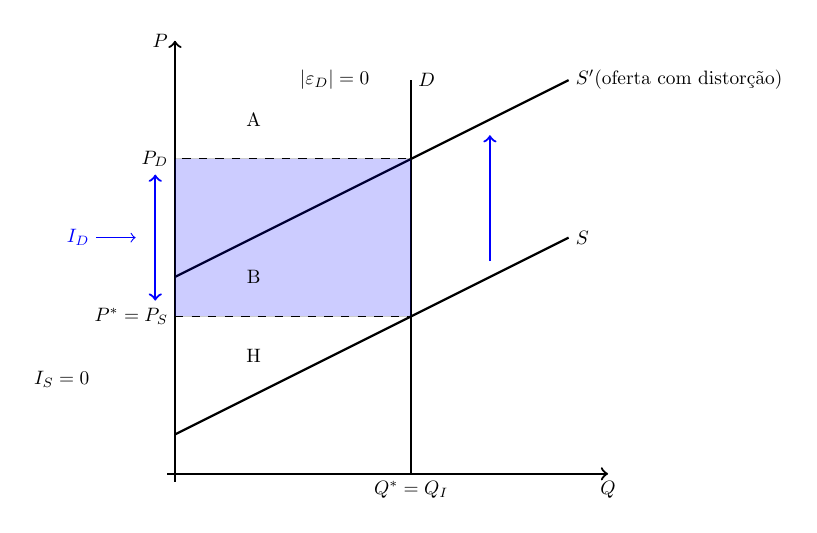
\begin{tikzpicture}[
			scale = 1,
			every node/.style = {scale = 0.7},
			declare function = {
				sa(\x) = 1/2 + 1/2 * \x;
				sb(\x) = 5/2 + 1/2 * \x;
				sc(\x) = 1/4 + 1/4 * \x;
				sd(\x) = 5/4 + 1/4 * \x;
			}]
			\def\eqa{3}
			\def\eqb{3}
			\def\eqc{3}
			\def\eqd{3}

			\draw[->,thick] (-0.1,0) -- (5.5,0)node[below]{$Q$};
			\draw[->,thick] (0,-0.1) -- (0,5.5)node[left]{$P$};

			\draw[thick] (3,0) node[below]{$Q^*=Q_I$} -- (3,5) node[right]{$D$};
			\draw[thick,domain=0:5,variable=\x] plot (\x,{sa(\x)})node[right]{$S$};

			\draw[->,thick,blue] ({\eqa+1},{sa(\eqa+1)+0.2}) -- ({\eqa+1},{sb(\eqa+1)-0.2}) node[midway,xshift=3cm]{};
			\draw[thick,domain=0:5,variable=\x] plot (\x,{sb(\x)})node[right]{$S'$(oferta com distor\c c\~ao)};

			\draw[dashed] (0,{sa(3)})node[left]{$P^*=P_S$} -- (3,{sa(3)}) -- (3,{sb(3)}) -- (0,{sb(3)})node[left]{$P_D$};
			\draw[fill=blue,opacity=0.2] (0,{sa(3)}) -- (3,{sa(3)}) -- (3,{sb(3)}) -- (0,{sb(3)});

			\draw(1.5,5)node[right]{\(|\varepsilon_D|=0\)};

			\draw[<->,blue,thick] (-0.25,{sa(3)+0.2}) -- (-0.25,{sb(3)-0.2});
			\draw[->,blue] (-1,{(sa(3)+sb(3))/2}) node[left]{$I_D$} -- (-0.5,{(sa(3)+sb(3))/2});
			\draw (-1,{(sa(3)+sb(3))/5}) node[left]{$I_S=0$};

			\draw(1,1.5)node[]{H};
			\draw(1,2.5)node[]{B};
			\draw(1,4.5)node[]{A};

		\end{tikzpicture}
	\end{center}
\end{frame}

\begin{frame}
	\frametitle{Impostos Indirectos}
	Com lan\c camento de imposto \emph{ad valorem} a 30\%
	\begin{align*}
		\left\{
			\begin{array}{c}
				Q_D=100-P_D\\
				Q_S=3P_S\\
				Q_D=Q_S\\
				P_D=P_S+0.3P_S
			\end{array}
		\right.
		\Leftrightarrow
		\left\{
			\begin{array}{c}
				Q_D=Q_S=69.77\\
				P_D=30.233\\
				P_S=23.256
			\end{array}
		\right.
	\end{align*}

	\begin{center}
		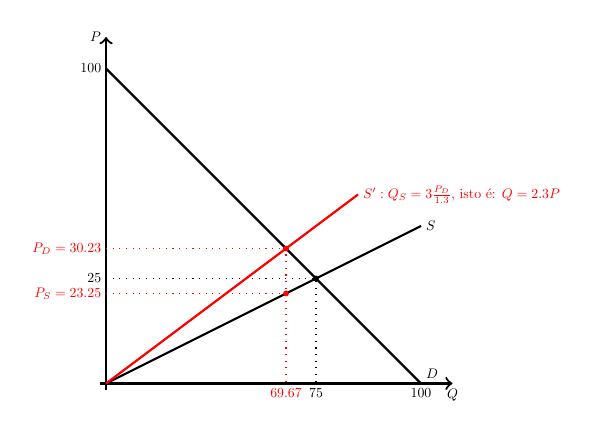
\begin{tikzpicture}[
			scale = 0.8,
			every node/.style = {scale = 0.5},
			declare function = {
				d(\x) = 5-\x;
				s(\x) = (1/2)*\x;
			}]

			\draw[->,thick] (-0.1,0) -- (5.5,0)node[below]{$Q$};
			\draw[->,thick] (0,-0.1) -- (0,5.5)node[left]{$P$};

			\draw[domain=0:5,variable=\x,thick] plot (\x,{d(\x)})node[above right]{$D$}node[below]{100};
			\draw[domain=0:5,variable=\x,thick] plot (\x,{s(\x)})node[right]{$S$};

			\draw(0,{d(0)}) node[left]{100};

			\draw[dotted] (0,{5/3})node[left]{25} -- ({10/3},{5/3})node[circle,fill,inner sep=1.5]{} -- ({10/3},0)node[below]{75};

			\draw[dotted,red] (0,{d(10/3.5)})node[left]{$P_D=30.23$} -- ({10/3.5},{d(10/3.5)}) node[circle,fill=red,inner sep=1.5]{} -- ({10/3.5},0)node[below]{69.67};
			\draw[dotted,red] (0,{s(10/3.5)})node[left]{$P_S=23.25$} -- ({10/3.5},{s(10/3.5)}) node[circle,fill=red,inner sep=1.5]{};

			\draw[domain=0:4,variable=\x,thick,red] plot (\x,{(d(10/3.5)/(10/3.5))*\x}) node[right]{$S':Q_S=3\frac{P_D}{1.3}$, isto \'e: $Q=2.3 P$};

		\end{tikzpicture}
	\end{center}

\end{frame}

\begin{frame}
	\frametitle{Impostos Indiretos (\emph{ad valorem} \`a taxa $t$)}
	\begin{center}
		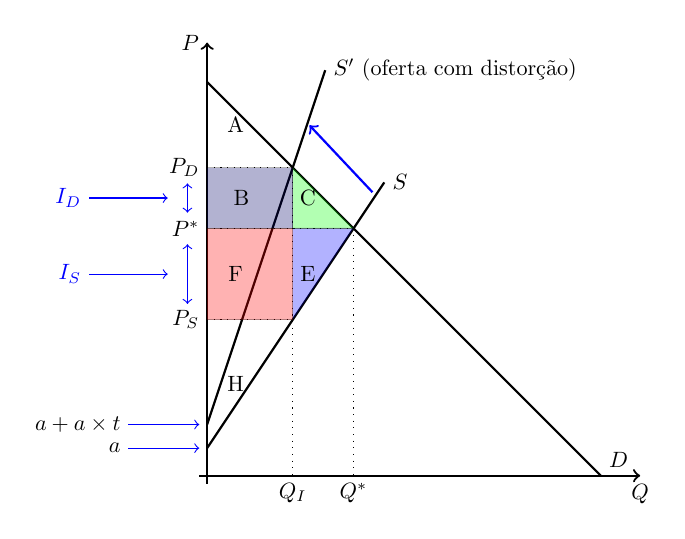
\begin{tikzpicture}[
			scale = 1,
			every node/.style = {scale = 0.8},
			declare function = {
				d(\x) = 5-\x;
				sa(\x) = 0.35+1.5*\x;
				sb(\x) = 0.65+3*\x;
				sc(\x) = 0.5+(1/2)*\x;
				sd(\x) = 0.5+(1/4)*\x;
			}]

			\def\eqa{93/50}
			\def\eqb{87/80}

			\draw[->,thick] (-0.1,0) -- (5.5,0)node[below]{$Q$};
			\draw[->,thick] (0,-0.1) -- (0,5.5)node[left]{$P$};

			\draw[domain=0:5,variable=\x,thick] plot (\x,{d(\x)})node[above right]{$D$}node[below]{};
			\draw[domain=0:2.25,variable=\x,thick] plot (\x,{sa(\x)})node[right]{$S$};
			\draw[domain=0:1.5,variable=\x,thick] plot (\x,{sb(\x)})node[right]{$S'$ (oferta com distor\c c\~ao)};
			\draw[blue,->] (-1,{sb(0)})node[text=black,left]{$a+a\times t$} -- (-0.1,{sb(0)});
			\draw[blue,->] (-1,{sa(0)})node[text=black,left]{$a$} -- (-0.1,{sa(0)});

			\draw[->,thick,blue] (2.1,{sa(2.1)+0.1}) -- (1.3,{sb(1.3)-0.1});

			\draw[dotted] (0,{sb(\eqb)})node[left]{$P_D$} -- (\eqb,{sb(\eqb)}) -- (\eqb,0)node[below]{$Q_I$};
			\draw[dotted] (0,{sa(\eqa)})node[left]{$P^*$} -- (\eqa,{sa(\eqa)}) -- (\eqa,0)node[below]{$Q^*$};
			\draw[dotted] (0,{sa(\eqb)})node[left]{$P_S$} -- (\eqb,{sa(\eqb)});

			\draw[blue,<->] (-0.25,{sa(\eqb)+0.2}) -- (-0.25,{sa(\eqa)-0.2});
			\draw[blue,<->] (-0.25,{sa(\eqa)+0.2}) -- (-0.25,{sb(\eqb)-0.2});
			\draw[blue,->] (-1.5,{(sa(\eqb)+sa(\eqa))/2})node[left]{$I_S$} -- (-0.5,{(sa(\eqb)+sa(\eqa))/2});
			\draw[blue,->] (-1.5,{(sa(\eqa)+sb(\eqb))/2})node[left]{$I_D$} -- (-0.5,{(sa(\eqa)+sb(\eqb))/2});

			\draw[fill=red,opacity=0.3] (0,{sa(\eqb)}) -- (\eqb,{sa(\eqb)}) -- (\eqb,{sa(\eqa)}) -- (0,{sa(\eqa)});
			\draw[fill=blue,opacity=0.3] (\eqb,{sa(\eqb)}) -- (\eqa,{sa(\eqa)}) -- (\eqb,{sa(\eqa)});
			\draw[fill=green,opacity=0.3] (\eqa,{sa(\eqa)}) -- (\eqb,{sa(\eqa)}) -- (\eqb,{sb(\eqb)});
			\draw[fill=blue!40!black,opacity=0.3] (0,{sa(\eqa)}) -- (\eqb,{sa(\eqa)}) -- (\eqb,{sb(\eqb)}) -- (0,{sb(\eqb)});

			\draw ({\eqb/3},{(sa(\eqb)+sa(\eqa))/2}) node[]{F};
			\draw ({\eqb/2.5},{(sb(\eqb)+sa(\eqa))/2}) node[]{B};
			\draw ({\eqb/3},{(sb(\eqb)+d(0))/2}) node[]{A};
			\draw ({\eqb/3},{(sa(\eqb)+sa(0))/2}) node[]{H};
			\draw ({\eqb+(\eqa-\eqb)/4},{(sa(\eqb)+sa(\eqa))/2}) node[]{E};
			\draw ({\eqb+(\eqa-\eqb)/4},{(sb(\eqb)+sa(\eqa))/2}) node[]{C};

		\end{tikzpicture}
	\end{center}
\end{frame}

\begin{frame}
	\frametitle{Subs\'idio espec\'ifico}
	Com lan\c camento de subs\'idio espec\'ifico de 10um:
	\begin{align*}
		\left\{
			\begin{array}{c}
				Q_D=100-P_D\\
				Q_S=3P_S\\
				Q_D=Q_S\\
				P_D=P_S-10
			\end{array}
		\right.
		\Leftrightarrow
		\left\{
			\begin{array}{c}
				Q_D=Q_S=82.5\\
				P_D=17.5\\
				P_S=27.5
			\end{array}
		\right.
	\end{align*}

	\begin{center}
		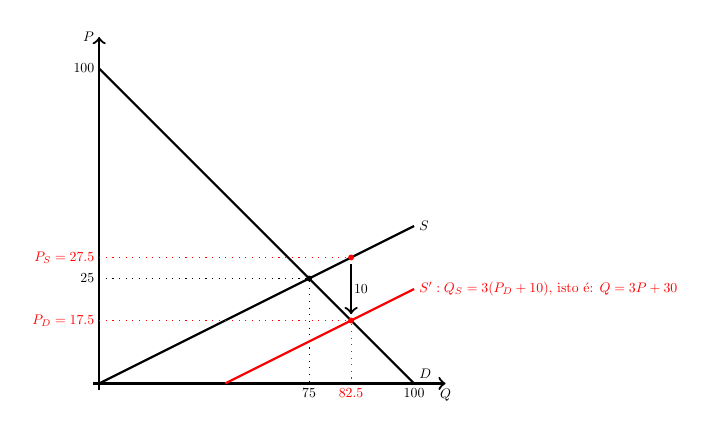
\begin{tikzpicture}[
			scale = 0.8,
			every node/.style = {scale = 0.5},
			declare function = {
				d(\x) = 5-\x;
				s(\x) = (1/2)*\x;
			}]

			\draw[->,thick] (-0.1,0) -- (5.5,0)node[below]{$Q$};
			\draw[->,thick] (0,-0.1) -- (0,5.5)node[left]{$P$};

			\draw[domain=0:5,variable=\x,thick] plot (\x,{d(\x)})node[above right]{$D$}node[below]{100};
			\draw[domain=0:5,variable=\x,thick] plot (\x,{s(\x)})node[right]{$S$};

			\draw(0,{d(0)}) node[left]{100};

			\draw[dotted] (0,{5/3})node[left]{25} -- ({10/3},{5/3})node[circle,fill,inner sep=1.5]{} -- ({10/3},0)node[below]{75};

			\onslide<2->{

				\draw[dotted,red] (0,{d(4)})node[left]{$P_D=17.5$} -- ({4},{d(4)}) node[circle,fill=red,inner sep=1.5]{};
				\draw[dotted,red] (0,{s(4)})node[left]{$P_S=27.5$} -- ({4},{s(4)}) node[circle,fill=red,inner sep=1.5]{} -- ({4},0)node[below]{82.5};

				\draw[domain=2:5,variable=\x,thick,red] plot (\x,{(s(\x-2)}) node[right]{$S':Q_S=3(P_D+10)$, isto \'e: $Q=3 P+30$};

			}

			\onslide<3->{
				\draw[->,thick] ({4},{s(4)-0.1}) -- ({4},{d(4)+0.1})node[midway,xshift=0.25cm]{$10$};
			}

		\end{tikzpicture}
	\end{center}
\end{frame}

\begin{frame}
	\frametitle{Subs\'idios}
	A perda excedente econ\'omico (perda pura, $C+E$), neste caso, \'e parte da despesa fiscal ($B+G+C+F+J+E$) que n\~ao \'e apropriada nem pelos consumidores (excedente $A+B+F+K$) nem pelos produtores (excedente $H+F+B+G$)
	\begin{center}
		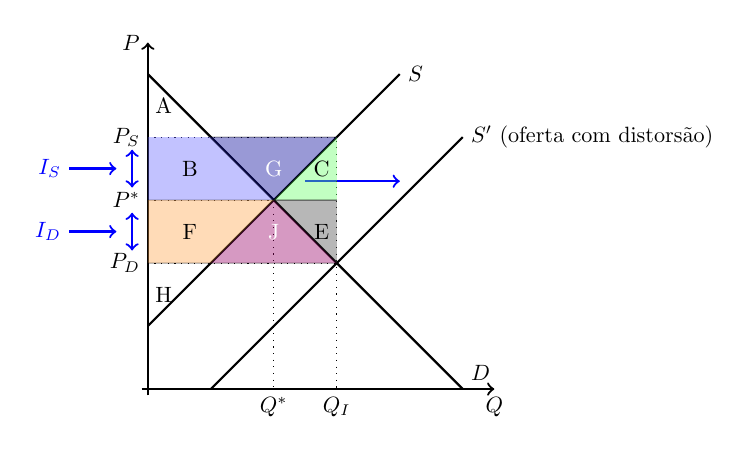
\begin{tikzpicture}[
			scale = 0.8,
			every node/.style = {scale = 0.8},
			declare function = {
				d(\x) = 5-\x;
				sa(\x) = 1+\x;
				sb(\x) = -1 + \x;
			}]

			\def\eqa{2}
			\def\eqb{3}

			\draw[->,thick] (-0.1,0) -- (5.5,0)node[below]{$Q$};
			\draw[->,thick] (0,-0.1) -- (0,5.5)node[left]{$P$};

			\draw[thick,domain=0:5,variable=\x] plot (\x,{d(\x)})node[above right]{$D$};
			\draw[thick,domain=0:4,variable=\x] plot (\x,{sa(\x)})node[right]{$S$};
			\draw[dotted] (0,{d(\eqa)})node[left]{$P^*$} -- (\eqa,{d(\eqa)}) -- (\eqa,0)node[below]{$Q^*$};

			\onslide<2>{
				\draw[->,blue,thick] ({\eqa+0.5},{sa(\eqa+0.3)}) -- ({\eqa+2},{sa(\eqa+0.3)});	
			}

			\onslide<2->{
				\draw[thick,domain=1:5,variable=\x] plot (\x,{sb(\x)})node[right]{$S'$ (oferta com distors\~ao)};	
			}

			\onslide<3->{
				\draw[dotted] (0,{sa(\eqb)})node[left]{$P_S$} -- (\eqb,{sa(\eqb)}) -- (\eqb,0)node[below]{$Q_I$};
				\draw[dotted] (0,{sb(\eqb)})node[left]{$P_D$} -- (\eqb,{sb(\eqb)});
			}

			\onslide<4->{
				\draw[blue,thick,<->] (-0.25,{sb(\eqb)+0.2}) -- (-0.25,{d(\eqa)-0.2});
				\draw[blue,thick,<->] (-0.25,{d(\eqa)+0.2}) -- (-0.25,{sa(\eqb)-0.2});
				\draw[blue,thick,->] (-1.25,{(sb(\eqb)+d(\eqa))/2})node[left]{$I_D$} -- (-0.5,{(sb(\eqb)+d(\eqa))/2});
				\draw[blue,thick,->] (-1.25,{(sa(\eqb)+d(\eqa))/2})node[left]{$I_S$} -- (-0.5,{(sa(\eqb)+d(\eqa))/2});
			}

			\onslide<5->{
				\draw[fill=blue!60!white,opacity=0.4] (0,{sa(\eqb)}) -- (0,{d(\eqa)}) -- (\eqa,{d(\eqa)}) -- (1,{sa(\eqb)});
				\draw[fill=blue!60!black,opacity=0.4] (1,{sa(\eqb)}) -- (\eqb,{sa(\eqb)}) -- (\eqa,{d(\eqa)});
				\draw[fill=green!60!white,opacity=0.4] (\eqb,{sa(\eqb)}) -- (\eqa,{d(\eqa)}) -- (\eqb,{sa(\eqa)});
				%\draw[fill=green!60!black,opacity=0.4] (\eqb,{sa(\eqa)}) -- (\eqa,{d(\eqa)}) -- (\eqb,{sb(\eqb)});
				\draw[fill=gray!60!black,opacity=0.4] (\eqb,{sa(\eqa)}) -- (\eqa,{d(\eqa)}) -- (\eqb,{sb(\eqb)});
				\draw[fill=red!60!blue,opacity=0.4] (\eqa,{d(\eqa)}) -- (\eqb,{sb(\eqb)}) -- (1,{sb(\eqb)});
				\draw[fill=orange!70!white,opacity=0.4] (\eqa,{sa(\eqa)}) -- (1,{sb(\eqb)}) -- (0,{sb(\eqb)}) -- (0,{sa(\eqa)});
			}

			\onslide<6->{
				\draw(0.25,{(d(0)+sa(\eqb))/2})node[]{A};
				\draw({\eqa/3},{(sa(\eqb)+sa(\eqa))/2})node[]{B};
				\draw({\eqa/3},{(sa(\eqa)+sb(\eqb))/2})node[]{F};
				\draw(0.25,{(sa(0)+sb(\eqb))/2})node[]{H};

				\draw[white](\eqa,{(d(1)+sa(\eqa))/2})node[]{G};
				\draw[white](\eqa,{(sa(1)+sa(\eqa))/2})node[]{J};
				
				\draw({\eqb*0.92},{(sa(\eqb)+sa(\eqa))/2})node[]{C};
				\draw({\eqb*0.92},{(sa(\eqa)+sb(\eqb))/2})node[]{E};
			}

		\end{tikzpicture}
	\end{center}
\end{frame}

\begin{frame}
	\frametitle{Em resumo}
	\begin{center}
		{
		\renewcommand{\arraystretch}{1.5}
		\footnotesize
		\begin{tabular}{ccc}
		\rowcolor{iscal_color}	& {\color{white}\textbf{Ap\'os subs\'idio}} & {\color{white}\textbf{Antes de subs\'idio}} \\
		\hline
		\rowcolor{iscal_color!10!white} Excedente de Consumidor 	& $A+B+F+J$ 	& $A+B$ \\
		\rowcolor{iscal_color!20!white} Excedente de Produtor 		& $F+H+B+G$ 	& $F+H$ \\
		\rowcolor{iscal_color!10!white} Despesa Fiscal (do Estado)  & $B+G+C+F+J+E$ & --\\
		\rowcolor{iscal_color!20!white} Perda Pura de Excedente 	& $C+E$ 		& -- \\
		\rowcolor{iscal_color!10!white} Quantidade Transacionada 	& $Q_I$ 		& $Q^*$ \\
		\rowcolor{iscal_color!20!white} Pre\c co Transac\c c\~ao 	& $P_D$; $P_S$  & $P^*$
		\end{tabular}

		\vspace{0.3cm}

		Incid\^encia Econ\'omica do subs\'idio, por unidade transacionada:\par $I_S(produtor)$; $I_D(consumidor)$
		}
	\end{center}
\end{frame}

\begin{frame}
	\frametitle{Em resumo}
	\begin{columns}
		\begin{column}{0.6\textwidth}
			\begin{center}
				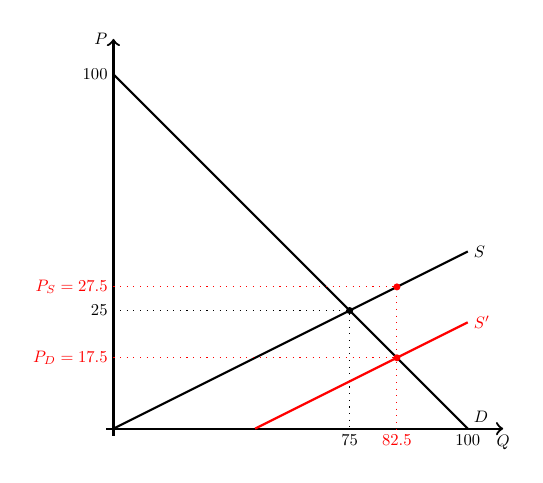
\begin{tikzpicture}[
					scale = 0.9,
					every node/.style = {scale = 0.6},
					declare function = {
						d(\x) = 5-\x;
						s(\x) = (1/2)*\x;
					}]

					\draw[->,thick] (-0.1,0) -- (5.5,0)node[below]{$Q$};
					\draw[->,thick] (0,-0.1) -- (0,5.5)node[left]{$P$};

					\draw[domain=0:5,variable=\x,thick] plot (\x,{d(\x)})node[above right]{$D$}node[below]{100};
					\draw[domain=0:5,variable=\x,thick] plot (\x,{s(\x)})node[right]{$S$};

					\draw(0,{d(0)}) node[left]{100};

					\draw[dotted] (0,{5/3})node[left]{25} -- ({10/3},{5/3})node[circle,fill,inner sep=1.5]{} -- ({10/3},0)node[below]{75};

					\draw[dotted,red] (0,{d(4)})node[left]{$P_D=17.5$} -- ({4},{d(4)}) node[circle,fill=red,inner sep=1.5]{};
					\draw[dotted,red] (0,{s(4)})node[left]{$P_S=27.5$} -- ({4},{s(4)}) node[circle,fill=red,inner sep=1.5]{} -- ({4},0)node[below]{82.5};

					\draw[domain=2:5,variable=\x,thick,red] plot (\x,{(s(\x-2)}) node[right]{$S'$};

				\end{tikzpicture}
			\end{center}
		\end{column}
		\begin{column}{0.4\textwidth}
			\begin{itemize}
				\item \(I_S=27.5-25=2.5um\)
				\item \(I_D=25-17.5=7.5um\)
				\item \(Total = 10um = I\)
			\end{itemize}
		\end{column}
	\end{columns}
\end{frame}